Las tablas que siguen muestran el promedio sobre las muestras disponibles
para cada tamaño. Tiempos en microsegundos, memoria en KB.

\begin{table}[H]
\centering
\caption{Tiempo promedio de sorting por tamaño (microsegundos).}
\label{tab:sorting-times}
\begin{tabular}{r|rrrr}
\hline
$n$ & MergeSort & QuickSort & PatienceSort & \texttt{std::sort}\\
\hline
10 & 0.78 & 0.00 & 1.67 & 0.44\\
$10^3$ & 46.94 & 173.50 & 452.61 & 11.28\\
$10^5$ & 5315.83 & 1434692.50 & 4711136.44 & 1518.11\\
$10^7$ & 1114715.50 & 666462.33$^*$ & 390309072.33 & 704833.00\\
\hline
\end{tabular}
\end{table}

\noindent$^*$Promedio de las tres muestras $D7$ (aleatorio). Se excluye a
propósito la muestra $D1,a$ de $n=10^7$: ahí QuickSort tardó
\textbf{3\,045\,046\,767~us (\textasciitilde50.8 minutos)}, casi tres órdenes
de magnitud más que en $D7$.

Con solo 10 valores distintos, tener el pivote fijo (siempre el primer
elemento) genera particiones desbalanceadas de manera sistemática, no por
casualidad, y el tiempo medido sigue casi al pie de la letra la curva de
referencia $O(n^2)$ que se ve en la Figura~\ref{fig:sorting-random}. De hecho
es el caso más claro de todo el experimento: la cota superior del peor caso
deja de ser algo teórico y se vuelve algo que uno observa directamente en los
números.

La Tabla~\ref{tab:sorting-times} deja claro que \texttt{std::sort} se
mantiene competitivo de forma consistente. En $10^5$, tanto QuickSort como
PatienceSort empeoran, sobre todo frente a entradas con valores repetidos o
parcialmente ordenadas --- un problema que se agrava mucho más en $10^7$ para
QuickSort dentro del dominio $D1$ (ver la nota anterior). Mirando solo $D7$,
PatienceSort tardó en promedio unos 390 segundos en $n=10^7$, muy por encima
del $O(n\log n)$ que sí logran \texttt{std::sort} y MergeSort. Las
Figuras~\ref{fig:sorting-random} y~\ref{fig:sorting-ordered} muestran estas
tendencias en escala logarítmica.

\begin{table}[H]
\centering
\caption{Memoria residente promedio registrada en sorting (KB).}
\label{tab:sorting-memory}
\begin{tabular}{r|rrrr}
\hline
$n$ & MergeSort & QuickSort & PatienceSort & \texttt{std::sort}\\
\hline
10 & 0 & 0 & 0 & 0\\
$10^3$ & 0 & 0 & 0 & 0\\
$10^5$ & 0 & 0 & 0 & 0\\
$10^7$ & 19520.00 & 0 & 38566.67 & 0\\
\hline
\end{tabular}
\end{table}

La memoria se estimó como la diferencia de \texttt{ru\_maxrss} antes y
después de cada algoritmo. Un valor de cero significa que no se detectó un
aumento del máximo residente en esa ejecución particular, no que el
algoritmo no use memoria adicional.

\begin{figure}[H]
\centering
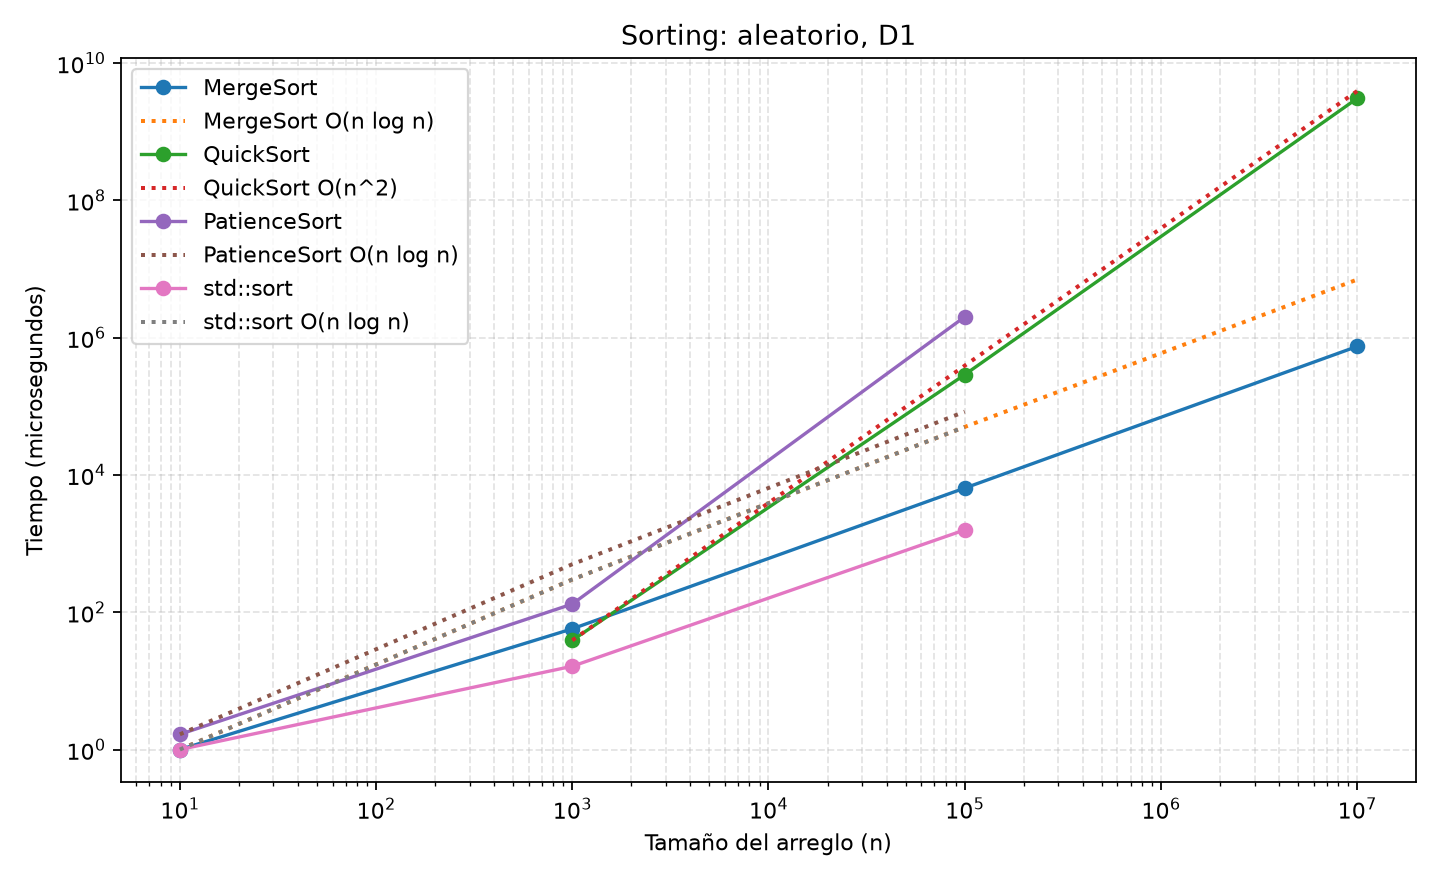
\includegraphics[width=0.84\textwidth]{../code/sorting/data/plots/generated_sorting_time_aleatorio_D1.png}
\caption{Sorting aleatorio en dominio $D1$.}
\label{fig:sorting-random}
\end{figure}

\begin{figure}[H]
\centering
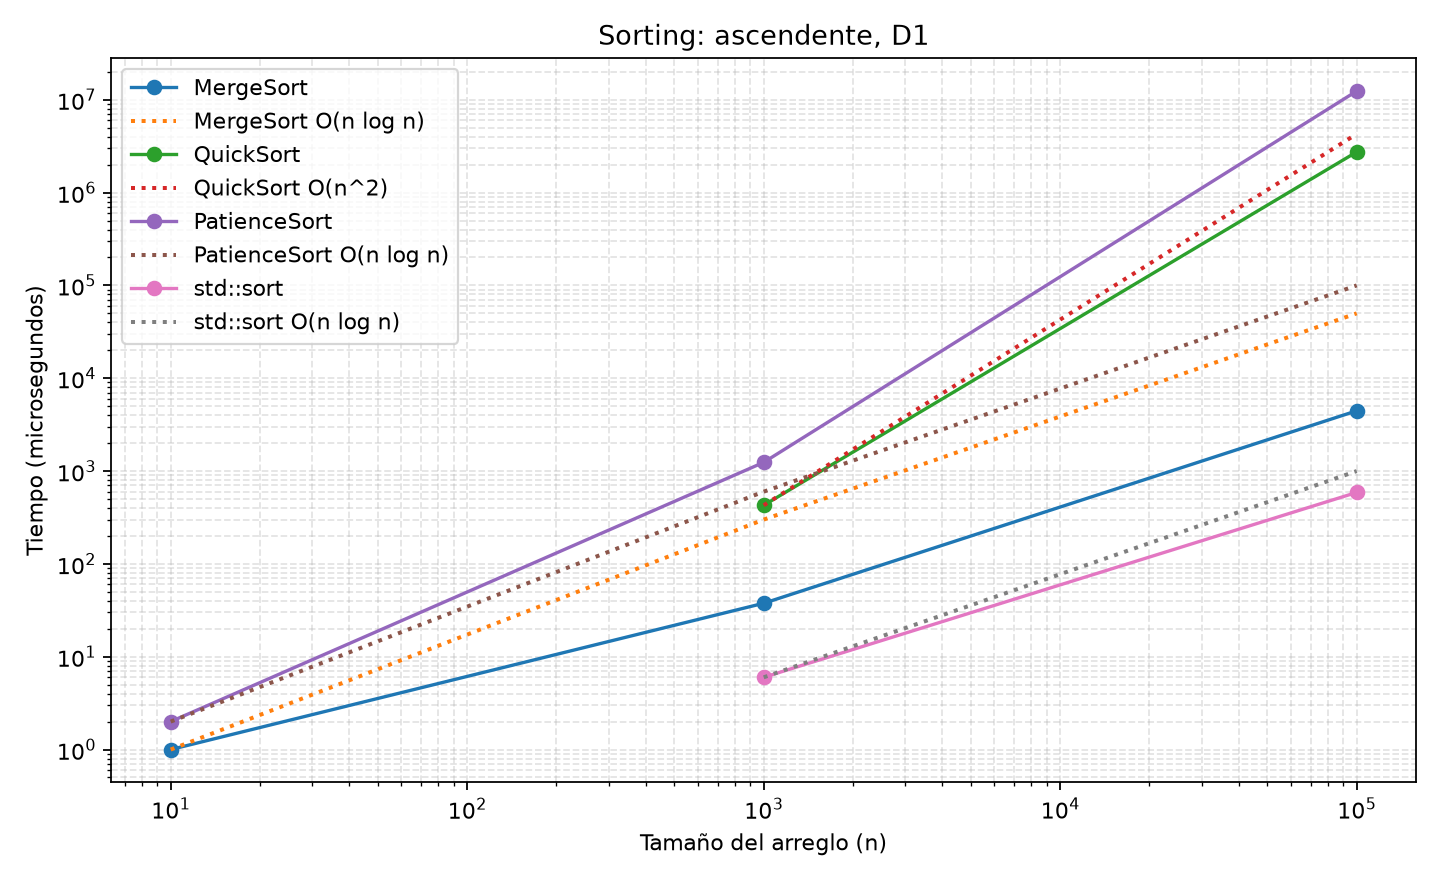
\includegraphics[width=0.84\textwidth]{../code/sorting/data/plots/generated_sorting_time_ascendente_D1.png}
\caption{Sorting ascendente en dominio $D1$.}
\label{fig:sorting-ordered}
\end{figure}

\begin{table}[H]
\centering
\caption{Tiempo promedio de multiplicación de matrices.}
\label{tab:matrix-times}
\begin{tabular}{r|rr}
\hline
$n$ & Naive & Strassen\\
\hline
16 & 1.72 & 519.11\\
64 & 92.50 & 23323.11\\
256 & 7236.06 & 1150298.44\\
1024 & 764579.33 & 55713463.44\\
\hline
\end{tabular}
\end{table}

En la Tabla~\ref{tab:matrix-times} se ve que Strassen termina siendo más caro
en este experimento, principalmente por sus constantes altas y por las
asignaciones y operaciones extra que arrastra. La diferencia se nota bien en
las Figuras~\ref{fig:matrix-dense} y~\ref{fig:matrix-diagonal}; en todos los
casos procesados, ambas implementaciones dieron matrices idénticas.

\begin{table}[H]
\centering
\caption{Memoria residente promedio registrada en matrices.}
\label{tab:matrix-memory}
\begin{tabular}{r|rr}
\hline
$n$ & Naive & Strassen\\
\hline
16 & 0 & 0\\
64 & 0 & 0\\
256 & 0 & 0\\
1024 & 0 & 1315.56\\
\hline
\end{tabular}
\end{table}

\begin{figure}[H]
\centering
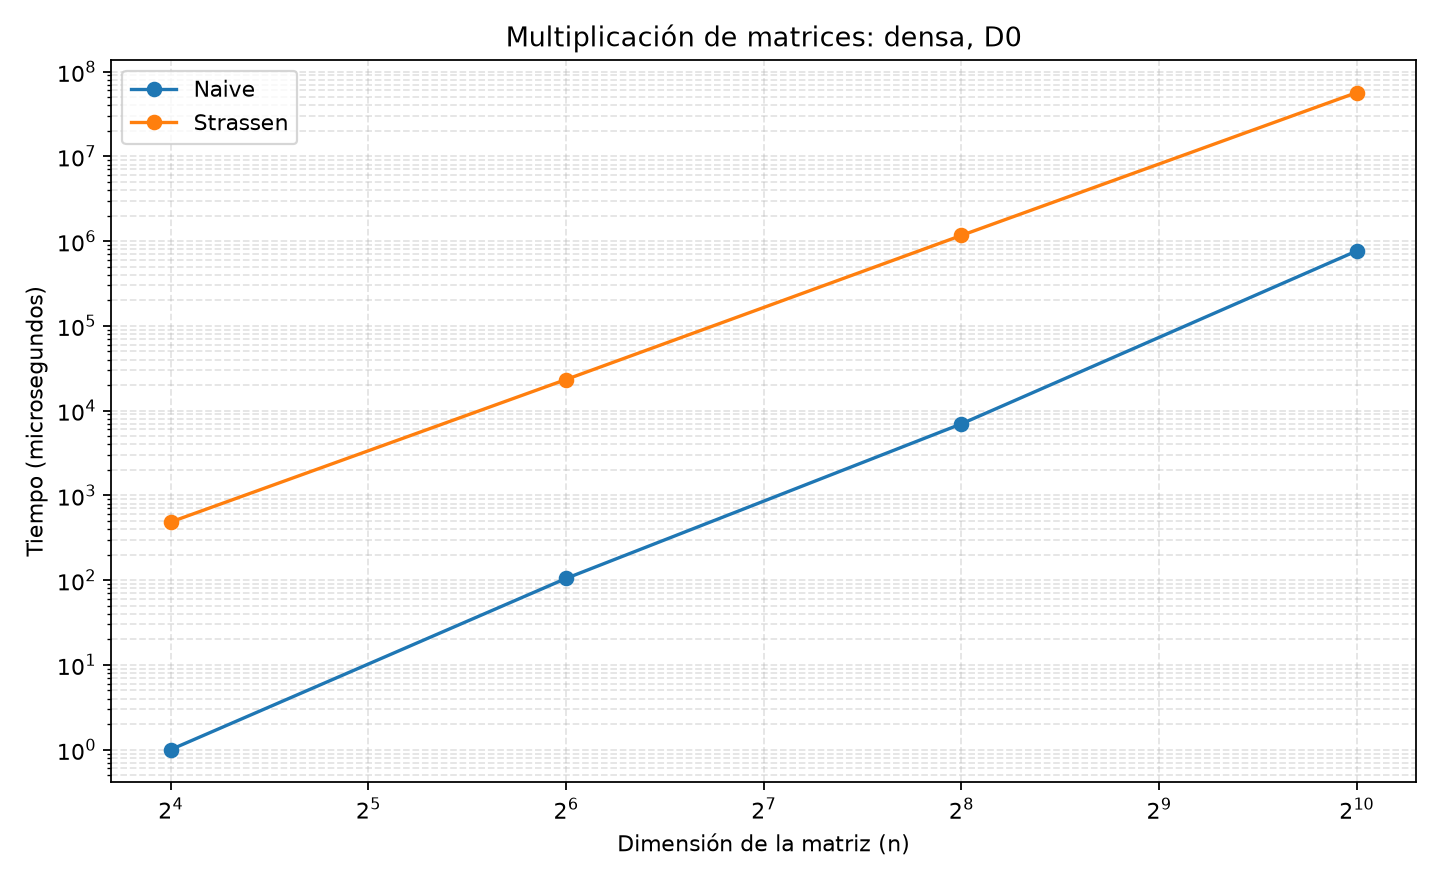
\includegraphics[width=0.84\textwidth]{../code/matrix_multiplication/data/plots/generated_matrix_time_densa_D0.png}
\caption{Multiplicación de matrices densas con dominio $D0$.}
\label{fig:matrix-dense}
\end{figure}

\begin{figure}[H]
\centering
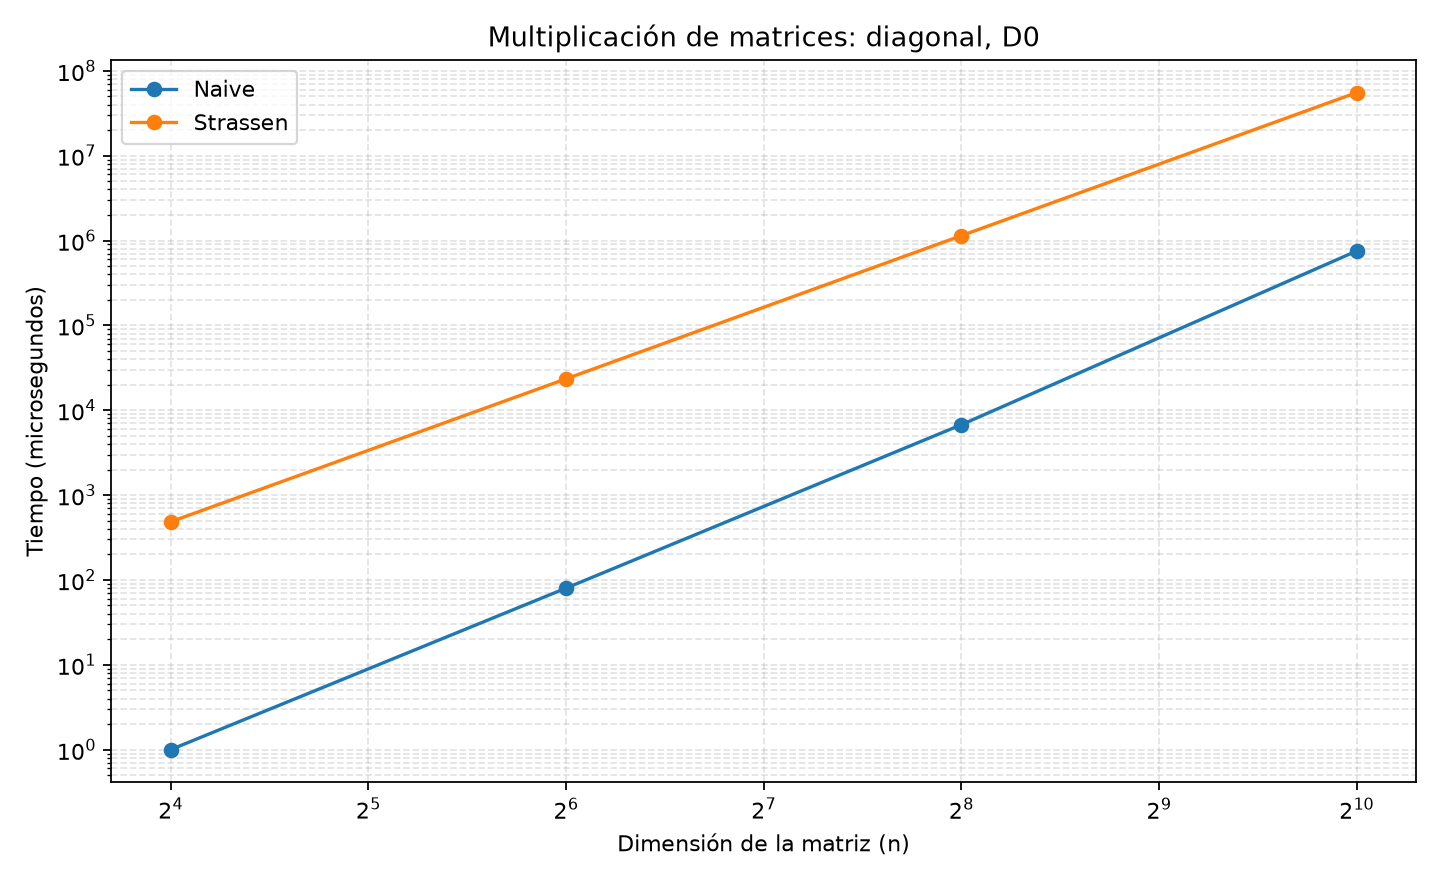
\includegraphics[width=0.84\textwidth]{../code/matrix_multiplication/data/plots/generated_matrix_time_diagonal_D0.png}
\caption{Multiplicación de matrices diagonales con dominio $D0$.}
\label{fig:matrix-diagonal}
\end{figure}

Las visualizaciones se generan automáticamente corriendo \texttt{make plot}
en cada directorio. Las figuras usadas están en
\url{code/sorting/data/plots/} y
\url{code/matrix_multiplication/data/plots/}.
